% Une ligne commentaire débute par le caractère « % »

\documentclass[a4paper]{article}

% Options possibles : 10pt, 11pt, 12pt (taille de la fonte)
%                     oneside, twoside (recto simple, recto-verso)
%                     draft, final (stade de développement)

\usepackage[utf8]{inputenc}   % LaTeX, comprends les accents !
\usepackage[T1]{fontenc}      % Police contenant les caractères français
\usepackage[francais]{babel}  


\usepackage[a4paper,left=2cm,right=2cm]{geometry}% Format de la page, réduction des marges
\usepackage{graphicx}  % pour inclure des images

%\pagestyle{headings}        % Pour mettre des entêtes avec les titres
                              % des sections en haut de page

 \title{  Qui est-ce ?\\         % Les paramètres du titre : titre, auteur, date
  Projet de programmation}          
\author{Groupe \emph{Z}\\
  \emph{Frédéric,Laurent,Tony et Romain}\\
  \emph{git:git@gitlab.etu.umontpellier.fr:e20180001091/qui-est-ce.git}\\
  L2 informatique\\
  Faculté des Sciences\\
Université de Montpellier.}
\date{\today}             


\begin{document}

\maketitle                    % Faire un titre utilisant les données
                              % passées à \title, \author et \date

\begin{center}               % pour centrer 
  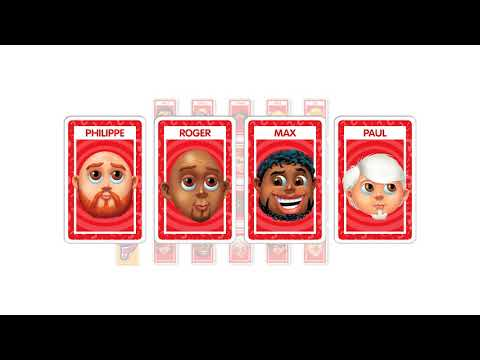
\includegraphics[scale=1]{img.jpg}   % insertion d'une image
\end{center}

\begin{abstract}     % Résumé du travail

  \emph{Description très succinte du problème et des différentes étapes de réalisation}

\end{abstract}


\section{Étape 3 : XXXX}

\emph{5 pages}

Description précise de l'extension réalisée - choix éventuels

Description de la résolution (protocole, algorithmes, ... selon l'extension choisie)


Extention "bot"

1er étape : Choisir la question
2e étape : Poser la question
3e étape : Mise à jour

Algorithme type glouton

Stratégie : Choisir la question qui recouvre le plus de personnages
Exemple : si 95 pourcent de nos personnages ont des cheveux noirs, 80 pourcent ont des yeux noirs et 10 pourcent ont un chapeau, l'agorithme posera la question "Est-ce que le personnage que je doit deviné a les cheveux noirs" en premier, "Est-ce que le personnage que je doit deviné a les yeux noirs" en deuxième puis une question pour le chapeau.

\end{document}